\section{Qué es un ser vivo}

Llamamos ser vivo a todo aquello que está formado por una o más células y realiza las tres funciones vitales: nutrición, relación y reproducción.

\subsection{Las células y sus tipos}
Una célula  (Figura \ref{fig:celula-eucariota}) es la parte más pequeña de un ser vivo que, a su vez, está viva; es decir, que puede realizar las funciones vitales; se nutre, se relaciona y se reproduce.

\vspace{3mm}
las células de diferentes seres vivos tienen una estructura común con cuatro componentes: la membrana, el citoplasma, el material genético y los orgánulos.

\begin{figure}[ht]
    \centering
    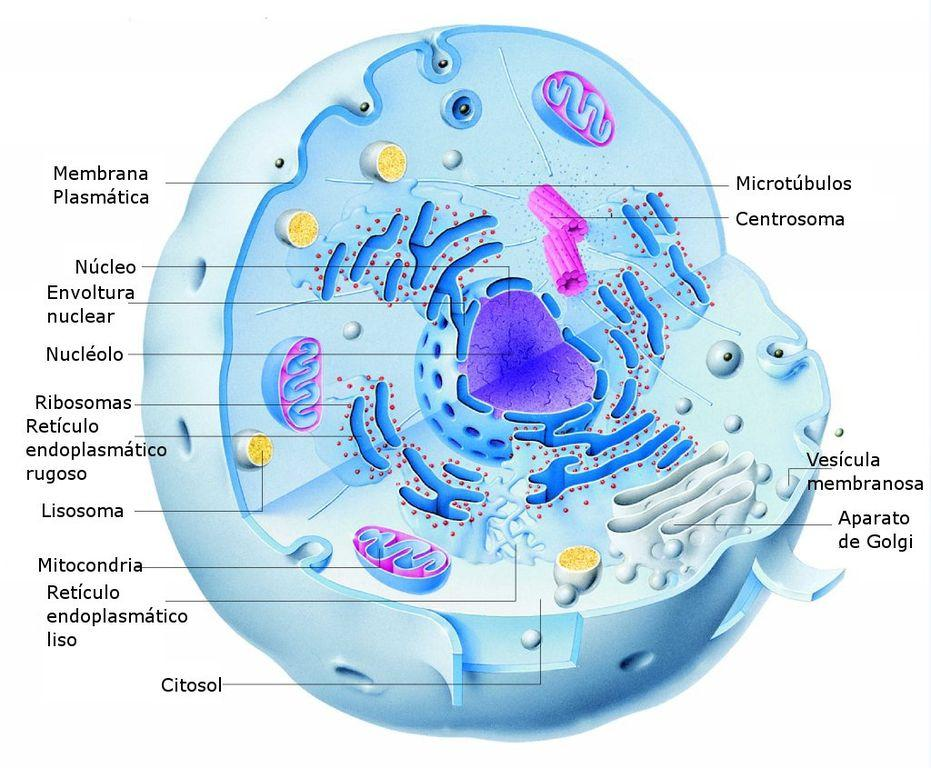
\includegraphics[width=0.7\linewidth]{Tema1/02_Celula_eucariota.jpg}
    \caption{Célula eucariota}
    \label{fig:celula-eucariota}
\end{figure}

\begin{itemize}
    \item \textbf{La membrana plasmática}, que es la envoltura fina y flexible que rodea a la célula y que regula el intercambio de sustancias con el exterior.
    \item \textbf{El citoplasma}, que es el gel que llena el interior de la célula.
    \item \textbf{El material genético}, que es la sustancia fibrosa llamada ADN que dirige el funcionamiento celular.
    \item \textbf{Los orgánulos}, que son estructuras especializadas en determinadas funciones. Según el tipo de células podremos encontrar unos orgánulos u otros.
\end{itemize}

Hay dos tipos principales de células, las \textbf{células procariotas} y las \textbf{células eucariotas}; Las células eucariotas se dividen en dos tipos: las \textbf{eucariotas de tipo animal} y las \textbf{eucariotas de tipo vegetal}.

\vspace{3mm}
Las células procariotas (Figura \ref{fig:celula-procariota}) tienen el material genético libre en el citoplasma, pocos orgánulos y una pared alrededor de la membrana.

\begin{figure}[ht]
    \centering
    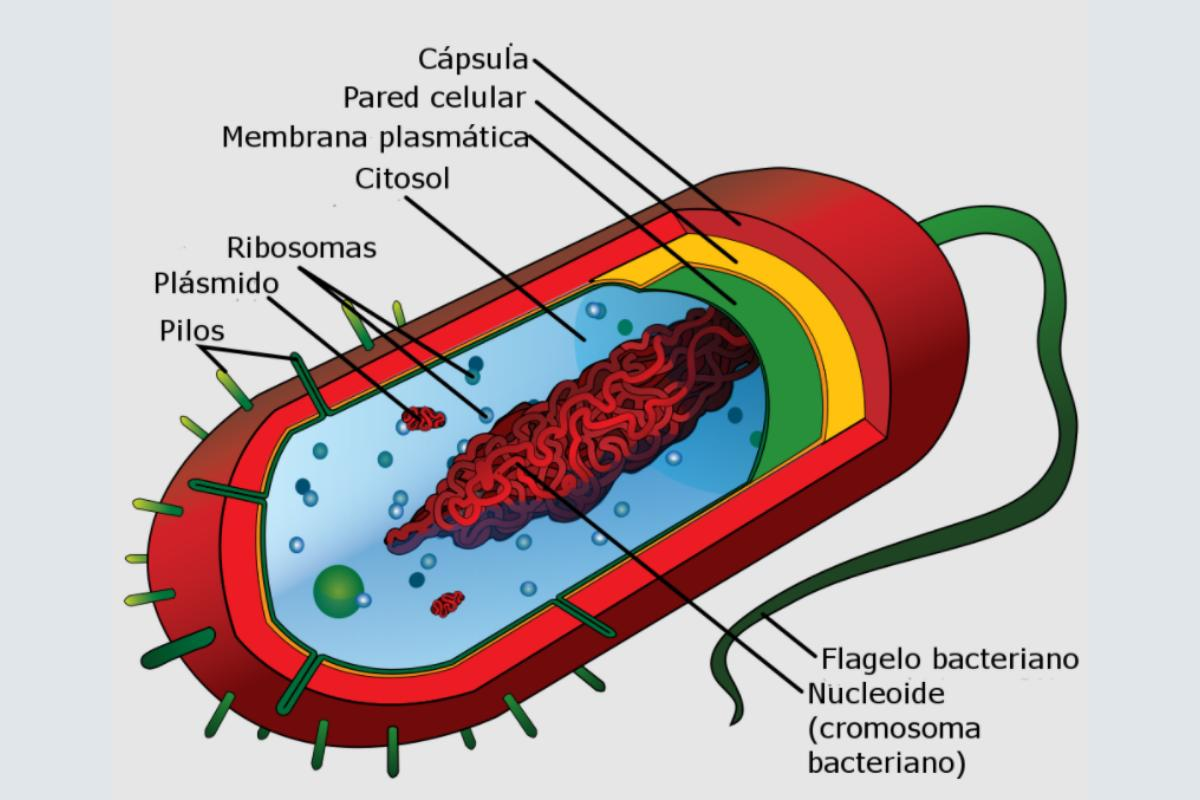
\includegraphics[width=0.6\linewidth]{Tema1/01_Celula_procariota.jpg}
    \caption{Célula procariota}
    \label{fig:celula-procariota}
\end{figure}

Las células eucariotas tienen el material genético rodeado de una membrana, que forma el núcleo, y se componen de una gran variedad de orgánulos.

\vspace{3mm}
Células eucariotas de tipo animal (Figura \ref{fig:eucariota-animal}) son las que tienen todos los animales y algunos organismos
como los protozoos.

\begin{figure}[ht]
    \centering
    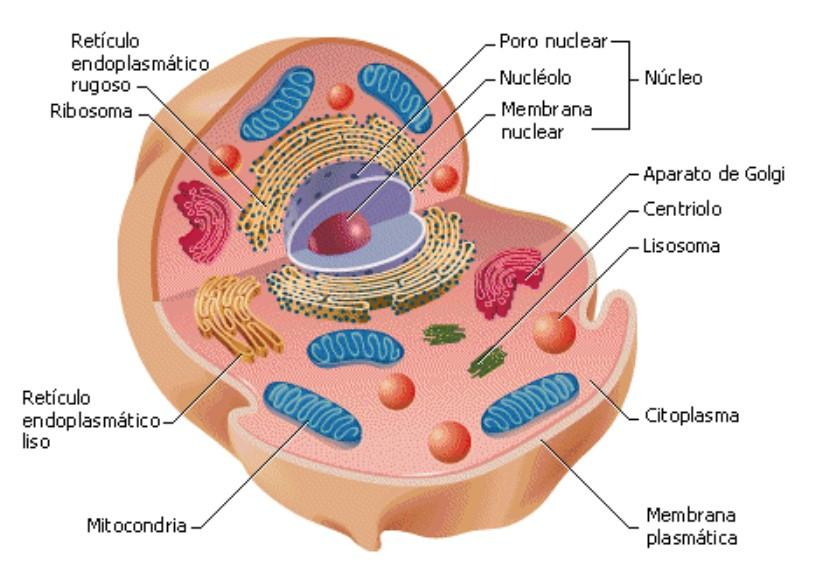
\includegraphics[width=0.6\linewidth]{Tema1/03_Celula_animal.jpg}
    \caption{Célula eucariota animal}
    \label{fig:eucariota-animal}
\end{figure}

\vspace{3mm}
Células eucariotas de tipo vegetal (Figura \ref{fig:eucariota-vegetal}) son las que tienen las plantas y las algas. Tienen una pared rígida y orgánulos especializados en realizar la fotosíntesis, como los cloroplastos.

\begin{figure}[!ht]
    \centering
    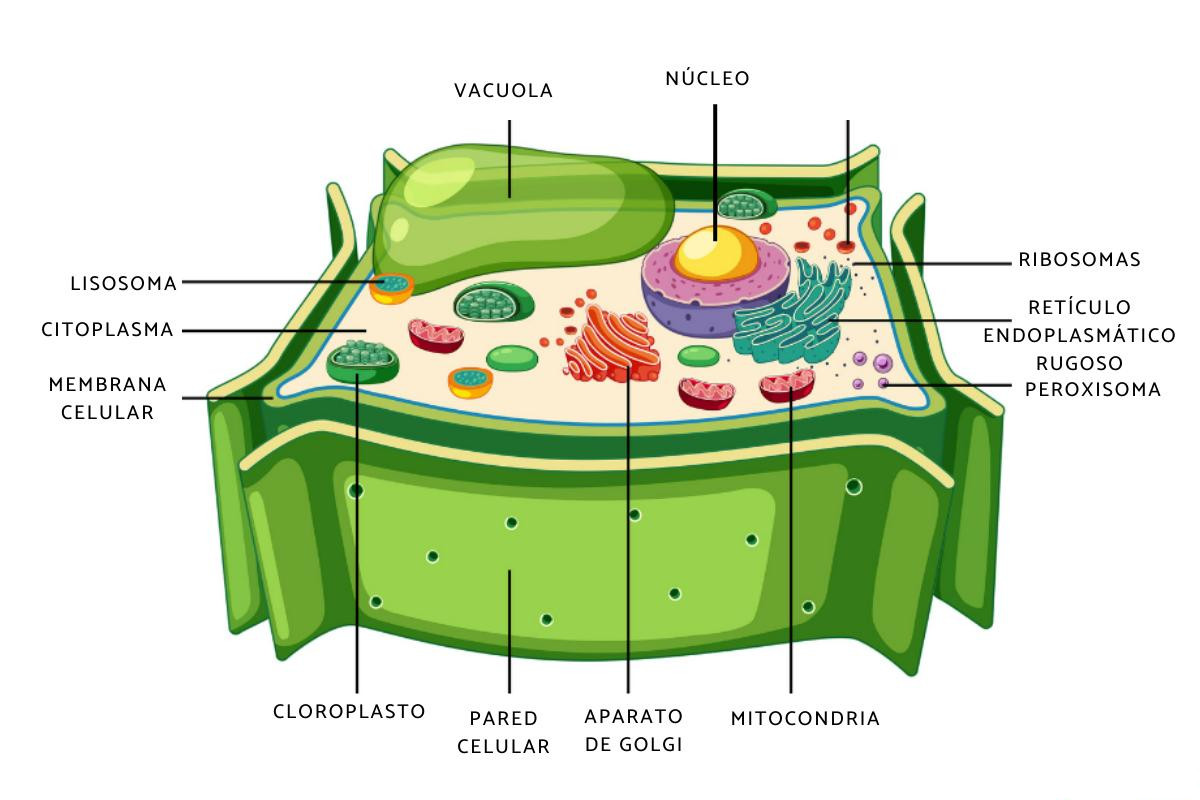
\includegraphics[width=0.7\linewidth]{Tema1/04_Celula_vegetal.jpg}
    \caption{Célula eucariota vegetal}
    \label{fig:eucariota-vegetal}
\end{figure}

\subsection{Las funciones vitales de las células}

Una célula es capaz de realizar las tres funciones vitales: nutrición, relación y reproducción.

\vspace{3mm}
\textbf{Función de nutrición} (Figura \ref{fig:nutricion-celular})

\begin{itemize}
    \item Consiguen nutrientes. Según la forma de obtener los nutrientes, la nutrición puede ser autótrofa o heterótrofa. Las células con nutrición autótrofa los fabrican con agua, dióxido de carbono y energía solar en un proceso llamado fotosíntesis. Las células con nutrición heterótrofa los obtienen de alimentos procedentes de otros seres vivos.
    \item Respiran. La mayoría de las células toman y utilizan el oxígeno del medio.
    \item Utilizan el alimento y el oxígeno. En su interior, las células utilizan los nutrientes y el oxígeno para crecer, para repararse y para obtener energía.
    \item Expulsan los desechos. Tras utilizar los nutrientes y el oxígeno, las células producen
sustancias de desecho que expulsan al exterior
a través de su membrana.
\end{itemize}

\begin{figure}[!ht]
    \centering
    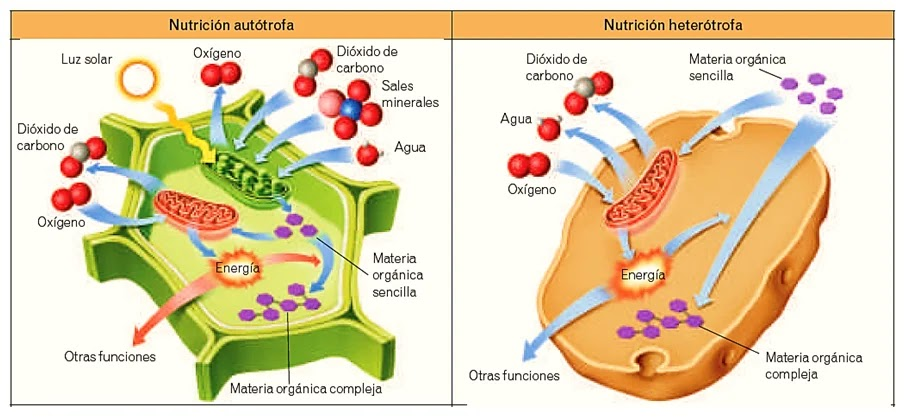
\includegraphics[width=0.8\linewidth]{Tema1/05_Nutricion_celular.jpg}
    \caption{Nutrición celular}
    \label{fig:nutricion-celular}
\end{figure}

\textbf{Función de relación} (Figura \ref{fig:relacion-celular})

Las células son capaces de reaccionar a cambios que se producen dentro o fuera de ella. Algunas son capaces de moverse y desplazarse gracias a ciertas partes especializadas.

\begin{figure}[!ht]
    \centering
    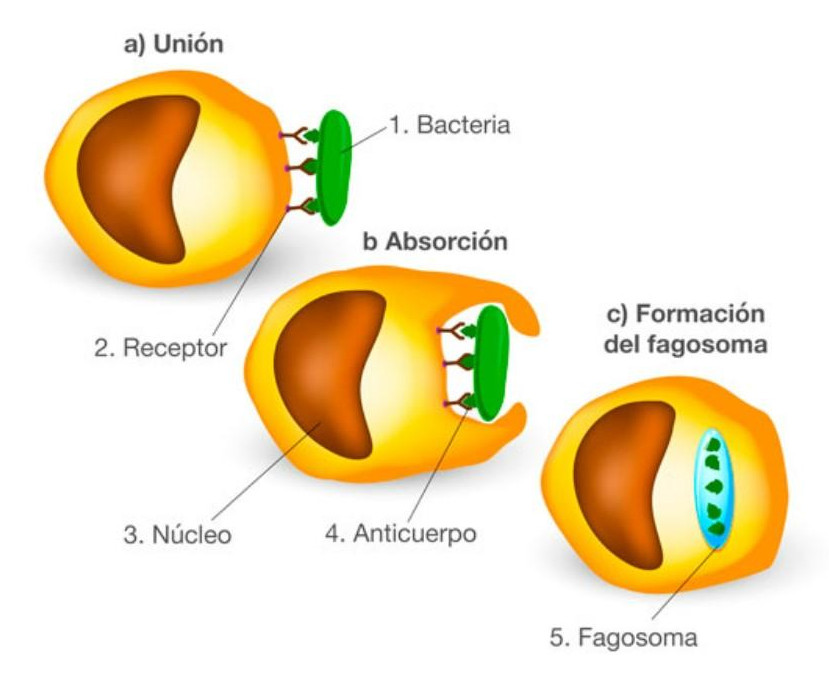
\includegraphics[width=0.5\linewidth]{Tema1/06_Relacion_celular.jpg}
    \caption{Función de relación}
    \label{fig:relacion-celular}
\end{figure}

\textbf{Función de reproducción} (Figura \ref{fig:reproduccion-celular}

Las células pueden formar células hija semejantes a ellas. Para ello, hacen una copia de su material genético y reparten su citoplasma en dos mitades. Material genético y citoplasma se separan y forman dos células.

\begin{figure}[!ht]
    \centering
    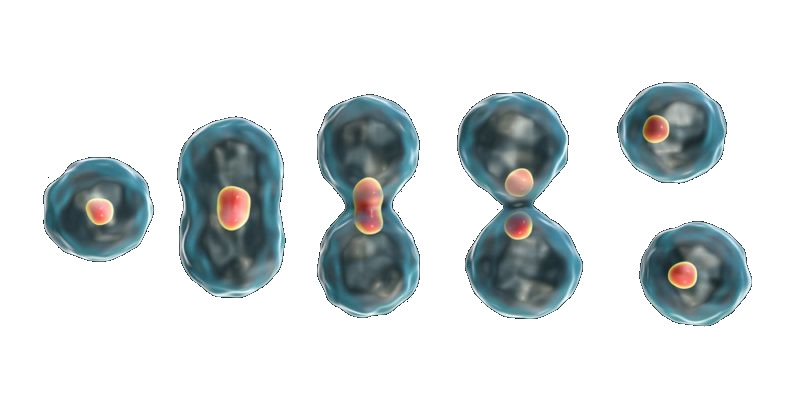
\includegraphics[width=0.6\linewidth]{Tema1/07_Reproduccion_celular.jpg}
    \caption{Función de reproducción}
    \label{fig:reproduccion-celular}
\end{figure}